\documentclass[12pt,a4paper]{article} 
\usepackage{tikz}
\usepackage{float}
\usepackage{graphicx}
\usepackage{multirow}
\usepackage{setspace} 
\usepackage{graphicx}
\usepackage{times}
\pagenumbering{roman}
\usepackage{geometry}

\geometry{verbose,tmargin=2cm,bmargin=2cm,lmargin=3cm,rmargin=2cm}
\usepackage{fancyhdr} 
%\linespread{1.05} 
\usepackage{tikz}
\usetikzlibrary{arrows}
\usetikzlibrary{shapes.geometric}

\tikzstyle{kres} = [rectangle, rounded corners, minimum width=1cm, minimum height=0.5cm,text centered, draw=black]
\tikzstyle{nad} = [trapezium, trapezium left angle=60, trapezium right angle=100, minimum width=1cm, minimum height=0.5cm, text centered, draw=black]
\tikzstyle{sim} = [trapezium, trapezium left angle=60, trapezium right angle=100, minimum width=1cm, minimum height=0.5cm, text centered, draw=black]
\tikzstyle{garis} = [thick,->,>=stealth]
\usetikzlibrary{shapes,arrows}

\begin{document} % Mulai Penulisan Laporan
\onehalfspacing
\begin{titlepage}

\title{\textbf{LAPORAN PRAKTIKUM ELEKTRONIKA DASAR
\\ RANGKAIAN DIODA }}  %Judul Laporan
%\title{\textbf{FOTOKATALISIS}}  %Judul Laporan
\author{\textbf {Dosen : Mada Sanjaya WS, Ph.D }
\\ \textbf{Asisten Lab : Dikha Khameswara (1177030010)}
\\ \textbf{ }
\\ \textbf{Disusun Oleh :}
\\ \textbf{Muhamad Fahmi Adzkar} \textbf {(1187030024)}
\\ \textbf{Kelompok 3 :}
\\ \textbf{Hani Hikmawati} \textbf {(1187030014)}
\\ \textbf{Sri Rahayu} \textbf {(1187030036)}
\\ \textbf{Yuni Rahayu} \textbf {(1187030041)}}

\maketitle
\begin{center}
\vspace{1cm}

\includegraphics[width=4cm]{uin.png}
\vspace{1cm}

JURUSAN FISIKA\\
FAKULTAS SAINS DAN TEKNOLOGI\\
UIN SUNAN GUNUNG DJATI BANDUNG\\
2019\\
\end{center}
\end{titlepage}

\renewcommand\abstractname{Abstract} %Untuk Abstrak Bahasa Inggris
\begin{abstract}
Alhamdulillah, in this experiment, we did an experiment for DIODA CIRCUIT.
A thermionic diode is a thermionic valve device which is an arrangement of electrodes in a vacuum in a glass cover. The first thermionic diode looks very similar to an incandescent light bulb. In a thermionic valve diode, electric current through the heating filament indirectly heats the cathode (Some diodes use direct heating, where the tungsten filament acts as a heater as well as a cathode), other internal electrodes are coated with a mixture of barium and strontium oxide, which is an oxide from alkaline earth metals. The substance was chosen because it has a small work function. The heat produced results in the thermionic emission of electrons into a vacuum. In advanced operation, the metal electrode next to the so-called anode is given a positive charge so that it electrostatically attracts the emitted electrons. However, electrons cannot be emitted easily from the surface of an anode that is not heated when the voltage polarity is reversed. Therefore, any reverse electricity generated can be ignored. For most of the 20th century, thermionic valve diodes were used in the use of analog signals, and as a rectifier in power boosters. At present, valve diodes are only used in special uses such as electric guitar amplifiers, high quality audio amplifiers and high voltage and power equipment.

\subparagraph{ }
\textit{Keywords: Diodes, resistor and capacitor circuits, resistance, voltage, electric current, transformer.}

\end{abstract}

\renewcommand\abstractname{Abstrak} %Untuk Abstrak Bahasa Indonesia
\begin{abstract}
	alhamdulillah pada percobaan kali ini kita melakukan percobaan untuk RANGKAIAN DIODA.
Dioda termionik adalah sebuah peranti katup termionik yang merupakan susunan elektrode-elektrode di ruang hampa dalam sampul gelas. Dioda termionik pertama bentuknya sangat mirip dengan bola lampu pijar. Dalam diode katup termionik, arus listrik yang melalui filamen pemanas secara tidak langsung memanaskan katode (Beberapa diode menggunakan pemanasan langsung, di mana filamen wolfram berlaku sebagai pemanas sekaligus juga sebagai katode), elektrode internal lainnya dilapisi dengan campuran barium dan strontium oksida, yang merupakan oksida dari logam alkali tanah. Substansi tersebut dipilih karena memiliki fungsi kerja yang kecil. Bahang yang dihasilkan menimbulkan pancaran termionik elektron ke ruang hampa. Dalam operasi maju, elektrode logam disebelah yang disebut anode diberi muatan positif jadi secara elektrostatik menarik elektron yang terpancar. Walaupun begitu, elektron tidak dapat dipancarkan dengan mudah dari permukaan anode yang tidak terpanasi ketika polaritas tegangan dibalik. Karenanya, aliran listrik terbalik apapun yang dihasilkan dapat diabaikan. Dalam sebagian besar abad ke-20, diode katup termionik digunakan dalam penggunaan isyarat analog, dan sebagai penyearah pada pemacu daya. Saat ini, diode katup hanya digunakan pada penggunaan khusus seperti penguat gitar listrik, penguat audio kualitas tinggi serta peralatan tegangan dan daya tinggi.alhamdulillah pada percobaan kali ini kita melakukan percobaan untuk RANGKAIAN DIODA.
Dioda termionik adalah sebuah peranti katup termionik yang merupakan susunan elektrode-elektrode di ruang hampa dalam sampul gelas. Dioda termionik pertama bentuknya sangat mirip dengan bola lampu pijar. Dalam diode katup termionik, arus listrik yang melalui filamen pemanas secara tidak langsung memanaskan katode (Beberapa diode menggunakan pemanasan langsung, di mana filamen wolfram berlaku sebagai pemanas sekaligus juga sebagai katode), elektrode internal lainnya dilapisi dengan campuran barium dan strontium oksida, yang merupakan oksida dari logam alkali tanah. Substansi tersebut dipilih karena memiliki fungsi kerja yang kecil. Bahang yang dihasilkan menimbulkan pancaran termionik elektron ke ruang hampa. Dalam operasi maju, elektrode logam disebelah yang disebut anode diberi muatan positif jadi secara elektrostatik menarik elektron yang terpancar. Walaupun begitu, elektron tidak dapat dipancarkan dengan mudah dari permukaan anode yang tidak terpanasi ketika polaritas tegangan dibalik. Karenanya, aliran listrik terbalik apapun yang dihasilkan dapat diabaikan. Dalam sebagian besar abad ke-20, diode katup termionik digunakan dalam penggunaan isyarat analog, dan sebagai penyearah pada pemacu daya. Saat ini, diode katup hanya digunakan pada penggunaan khusus seperti penguat gitar listrik, penguat audio kualitas tinggi serta peralatan tegangan dan daya tinggi.

\subparagraph{ }
\textit{Kata Kunci: Dioda, rangkaian resistor dan kapasitor, hambatan, tegangan, arus listrik, Tranformator.}

\end{abstract}

\newpage
\section{PENDAHULUAN}
\paragraph{1.1 Latar Belakang}
\subparagraph{ }
	Dalam sebuah rangkaian listrik dikenal dengan istilah arus listrik (I), tegangan atau beda potensial (V) dan hambatan (R). Pada dasarnya sebuah rangkaian listrik terjadi ketika sebuah penghantar mampu dialiri electron bebas secara terus menerus. Aliran inilah yang disebut dengan arus. Sedangkan tegangan adalah beda potensial yang ada di antara titik rangkaian listrik tersebut. Untuk menemukan hubungan di antara istilah-istilah yang ada dalam sebuah rangkaian listrik diperlukan sebuah praktikum yang dapat membuktikannya.
\subparagraph{ }
	Dengan melakukan praktikum yang berjudul RANGKAIAN DIODA ini kita dapat mengetahui dan mempelajari hubungan antara tegangan atau beda potensial dan kuat arus pada suatu rangkaian penyearah arus (setengah gelombang, satu gelombang penuh dan metode bridge)dan dapat digunakan untuk mengetahui sebuah sinyal output listrik tanpa harus menggunakan alat (multimeter). Selain itu materi tentang RANGKAIAN DIODA ini sangat berguna khususnya yang mendalami kelistrikan. Dan juga rangkaian penyearah ini sangat berhubungan dengan alat-alat otomatis yang terjadi disekitar kita, salah satunya sensor cahaya atau Light Dependent Resistor (LDR) yang sangat bermanfaat bagi kehidupan manusia.
 

\paragraph{1.2 Tujuan}
\subparagraph{ }
Adapun tujuan dilakukannya praktikum ini yaitu:
\begin{enumerate}
\item Mampu memahami yste dan prinsip kerjanya sebagai penyearah arus.
\item Mampu merancang penyearah gelombang ( setengah gelombang, satu gelombang penuh dan metode bridge ).
\item Mampu menganalisis dan menghitung bentuk gelombang output dari rangkaian penyearah gelombang ( setengah gelombang, satu gelombang penuh dan metode bridge ).
\end{enumerate}


\newpage
\section{Landasan Teori}
\subsection{Dasar Teori}
\paragraph{ }
\textbf{Dioda (komponen elektronik)}
	\subparagraph{ }
	Dioda adalah komponen aktif dua kutub yang pada umumnya bersifat semikonduktor, yang memperbolehkan arus listrik mengalir ke satu arah (kondisi panjar maju) dan menghambat arus dari arah sebaliknya (kondisi panjar mundur). Diode dapat disamakan sebagai fungsi katup di dalam bidang elektronika. Diode sebenarnya tidak menunjukkan karakteristik kesearahan yang sempurna, melainkan mempunyai karakteristik hubungan arus dan tegangan kompleks yang tidak linier dan seringkali tergantung pada teknologi atau material yang digunakan serta parameter penggunaan. Beberapa jenis diode juga mempunyai fungsi yang tidak ditujukan untuk penggunaan penyearahan.
	\subparagraph{ }
	Walaupun diode kristal (semikonduktor) dipopulerkan sebelum diode termionik, diode termionik dan diode kristal dikembangkan secara terpisah pada waktu yang bersamaan. Prinsip kerja dari diode termionik ditemukan oleh Frederick Guthrie pada tahun 1873 Sedangkan prinsip kerja diode kristal ditemukan pada tahun 1874 oleh peneliti Jerman, Karl Ferdinand Braun. Pada waktu penemuan, peranti seperti ini dikenal sebagai penyearah (rectifier). Pada tahun 1919, William Henry Eccles memperkenalkan istilah diode yang berasal dari di berarti dua, dan ode berarti "jalur".
	\subparagraph{ }
	Prinsip kerja diode termionik ditemukan kembali oleh Thomas Edison pada 13 Februari 1880 dan dia diberi hak paten pada tahun 1883 (U.S. Patent 307.031), namun tidak dikembangkan lebih lanjut. Braun mematenkan penyearah kristal pada tahun 1899. Penemuan Braun dikembangkan lebih lanjut oleh Jagdish Chandra Bose menjadi sebuah peranti berguna untuk detektor radio.
\subparagraph{ }
	Dioda termionik adalah sebuah peranti katup termionik yang merupakan susunan elektrode-elektrode di ruang hampa dalam sampul gelas. Dioda termionik pertama bentuknya sangat mirip dengan bola lampu pijar. Dalam diode katup termionik, arus listrik yang melalui filamen pemanas secara tidak langsung memanaskan katode (Beberapa diode menggunakan pemanasan langsung, di mana filamen wolfram berlaku sebagai pemanas sekaligus juga sebagai katode), elektrode internal lainnya dilapisi dengan campuran barium dan strontium oksida, yang merupakan oksida dari logam alkali tanah. Substansi tersebut dipilih karena memiliki fungsi kerja yang kecil. Bahang yang dihasilkan menimbulkan pancaran termionik elektron ke ruang hampa. Dalam operasi maju, elektrode logam disebelah yang disebut anode diberi muatan positif jadi secara elektrostatik menarik elektron yang terpancar. Walaupun begitu, elektron tidak dapat dipancarkan dengan mudah dari permukaan anode yang tidak terpanasi ketika polaritas tegangan dibalik. Karenanya, aliran listrik terbalik apapun yang dihasilkan dapat diabaikan. Dalam sebagian besar abad ke-20, diode katup termionik digunakan dalam penggunaan isyarat analog, dan sebagai penyearah pada pemacu daya. Saat ini, diode katup hanya digunakan pada penggunaan khusus seperti penguat gitar listrik, penguat audio kualitas tinggi serta peralatan tegangan dan daya tinggi.
\begin{flushright}
(WIKIPEDIA, 2019 7 OCTOBER 23:40) 
\end{flushright}
\paragraph{ }
	\textbf{Transformator Penurun Tegangan}
\subparagraph{ }
	\begin{figure}
	
	\end{figure}
	Transformator atau trafo adalah alat yang memindahkan tenaga listrik antar dua rangkaian listrik atau lebih melalui induksi elektromagnetik.Transformator bekerja berdasarkan prinsip induksi elektromagnetik. Tegangan masukan bolak-balik yang membentangi primer menimbulkan fluks magnet yang idealnya semua bersambung dengan lilitan sekunder. Fluks bolak-balik ini menginduksikan gaya gerak listrik (ggl) dalam lilitan sekunder. Jika efisiensi sempurna, semua daya pada lilitan primer akan dilimpahkan ke lilitan sekunder.Transformator step-up adalah transformator yang memiliki lilitan sekunder lebih banyak daripada lilitan primer, sehingga berfungsi sebagai penaik tegangan. Transformator ini biasa ditemui pada pembangkit tenaga listrik sebagai penaik tegangan yang dihasilkan generator menjadi tegangan tinggi yang digunakan dalam transmisi jarak jauh.
\begin{flushright}
(Haliday, 2010 hal: 179) 
\end{flushright}

\paragraph{ }
	\textbf{Rangkaian Penyearah Setengah Gelombang}
\subparagraph{ }
	Penyearah Setengah Gelombang (half wave rectifier) adalah sistem penyearah yang menggunakan satu blok dioda tunggal (bisa satu dioda atau banyak dioda yang diparalel) untuk mengubah tegangan dengan arus bolak-balik (AC) menjadi tegangan dengan arus searah (DC). Keluaran dari penyearah ini memiliki riak lebih besar dari penyearah gelombang penuh. Prinsip kerja dari rangkaian ini adalah  memanfaatkan karakteristik dioda yang hanya bisa dilalui arus satu arah saja. Disebut penyearah setengah gelombang karena penyearah ini hanya melewatkan siklus positif dari sinyal AC. Rangkaian penyearah setengah gelombang banyak dipakai pada power supply dengan frekuensi tinggi seperti pada power supply SMPS dan keluaran transformator Flyback Televisi.Penyearah sistem setengah gelombang kurang baik diaplikasikan pada frekuensi rendah seperti jala-jala listrik rumah tangga dengan frekuensi 50Hz. Hal ini disebabkan rangkaian akan membuang satu siklus sinyal AC dan mempunyai riak (ripple) yang besar pada keluaran tegangan DC-nya sehingga membutuhkan kapasitor yang besar.
\subparagraph{ }
	\textbf{Prinsip kerja Penyearah Setengah Gelombang}
\subparagraph{ }
	Contoh rangkaian penyearah setengah gelombang digambarkan pada ilustrasi gambar dibawah ini. Tegangan input dengan arus bolak-balik melewati satu dioda penyearah kemudian pada outputnya tampak melewatkan “gunung” dari sinyal sinus dan menghambat fase “lembah”-nya. Hal ini mengakibatkan keluaran dari penyearah jenis ini memiliki banyak riak (riple) dan membutuhkan kapasitor yang besar untuk meng-“halus”-kannya.Perhitungan tegangan DC keluaran dari penyearah setengah gelombang mengacu pada kondisi saat fasa on dan off pada gelombang output. Pada saat fase positif, dioda menghantar sehingga tegangan keluaran saat itu sama dengan Vmax dari sinyal input. Kemudian saat fase negatif, dioda tidak menghantar sehingga tegangan keluaran pada fase ini sama dengan nol.Berdasarkan kondisi diatas maka dapat dirumuskan bahwa besarnya tegangan output dari rangkaian penyearah adalah Vmax dibagi dengan (pi). Dimana besarnya Vmax adalah tegangan puncak (V-peak) dari salah satu siklus sinyal AC. Atau sebesar 0.318Vmax. Dan jika dihitung dengan nilai RMS menjadi 0.318 kali sqrt2 sama dengan 0.45Vrms.

\begin{flushright}
	(Soedojo, 2004 hal: 171) 
\end{flushright}

\paragraph{{Rangkaian Penyearah Gelombang Penuh Dengan Dua Dioda} }
\subparagraph{ }
	Penyearah Gelombang Penuh adalah sistem penyearah yang menyearahkan semua siklus gelombang sinus. Ada dua jenis penyearah gelombang penuh yaitu jenis penyearah dua dioda dan penyearah sistem jembatan. Pada artikel ini akan khusus dibahas penyearah gelombang penuh dengan sistem dua dioda. Sedangkan untuk penyearah sistem jembatan akan dibahas pasa artikel selanjutnya tentang dioda bridge.
	Komponen utama dari penyearah ini adalah dua blok dioda, dimana satu blok dioda bisa berupa satu atau beberapa dioda yang diparalel yang bekerja secara komplenen. Satu dioda bekerja pada fase siklus positif dan satu dioda bekerja pada fase siklus negatif yang telah dibalik.
	Oleh karena itu penyearah gelombang penuh identik dengan penggunaan jenis transformator center tap (CT) yang memiliki dua buah output sinyal AC dengan fase berkebalikan. Rangkaian penyearah dengan output gelombang penuh menghasilkan tegangan DC dengan riak (ripple) yang lebih sedikit dibanding penyearah setengan gelombang.
	Hal ini karena gelombang yang dihasilkan lebih rapat yaitu hasil penggabungan dari siklus sinyal sinus positif dan siklus sinyal sinus negatif yang telah dibalik menjadi siklus positif. Jadi penyearah akan tetap mengeluarkan output pada periode gunung dan lembah dari sinyal sinus.
\paragraph{ }
		\textbf{Prinsip Kerja Penyearah Gelombang Penuh}
\subparagraph{ }
	Prinsip kerja rangkaian penyearah gelombang penuh menyearahkan output dari sebuah transformator CT yang memiliki fasa berbeda menggunakan dua dioda penyearah. Gambar dibawah adalah contoh rangkaian penyearah gelombong penuh dengan dua dioda. Penyearah jenis ini memerlukan input dari sebuah transformer khusus yang memiliki tap tengah dan lazim disebut dengan Transformator CT (Centre Tapped).Dengan dua sinyal AC yang saling berbeda fase ini maka kedua dioda yang masing-masing berfungsi sebagai penyearah setengah gelombang dapat bekerja secara bergantian. 
	
	\begin{figure}
	\begin{center}
	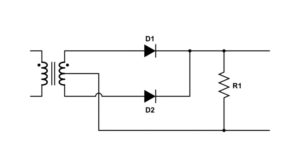
\includegraphics[width=6cm, height=3cm]{g1dt.png}
	\end{center}
	\end{figure}

	Satu dioda menyearahkan siklus positif dari lilitan atas. Kemudian satu dioda kemudian ganti menyearahkan siklus positif dari lilitan bawah yang merupakan balikan fasa dari siklus negatif sinyal input AC.
	Output dari penyearah yang lebih rapat dari penyearah setengah gelombang. Ini berarti lebih baik karena riak (ripple) yang ada pada output tegangan DC menjadi lebih kecil. Akibatnya output dari penyearah tersebut menjadi lebih halus dan lebih stabil dari penyearah setengah gelombang.

Perhitungan tegangan DC pada output rangkaian full-wave rectifier bisa dikatakan dua kali dari penyearah setengah gelombang. Hal ini karena semua siklus sinyal AC dikeluarkan. Jadi besarnya tegangan output dari rangkaian penyearah adalah 2 kali Vmax dibagi dengan (pi).

Dimana besarnya Vmax adalah tegangan puncak (V-peak) dari salah satu siklus sinyal AC. Atau sebesar 0.637Vmax. Dan jika dihitung dengan nilai RMS menjadi 0.637 kali sqrt2 sama dengan 0.9Vrms.

\begin{flushright}
	(Haliday, 2010 hal: 179)
\end{flushright}

\newpage
\section{METODE PRAKTIKUM}
\subsection{Waktu dan Tempat}
\paragraph{ }
Praktikum ini dilaksanakan pada:
\\ 		Tanggal : jum'at, 4 Oktober 2019
\\ 		Waktu : 07.00 WIB - Selesai
\\ 		Tempat : Advance Physics 

\subsection{Alat dan Bahan}
Alat dan bahan yang digunakan dalam praktikum ini diantaranya adalah : 
\subparagraph*{ }
\begin{tabular}{|l|l|l|}  \hline
No & Alat dan Bahan  & Jumlah  \\ \hline
1  & PCB matriks & 3 buah \\ \hline
2  & Multimeter & 1 buah \\ \hline
3  & Osiloskop & 1 buah \\ \hline
4  & Kabel Peenghubung & Secukupnya \\ \hline
5  & Transformator & 1 buah \\ \hline
6  & Dioda & 7 buah \\ \hline
7  & Resistor & 3 buah \\ \hline
8  & Kapasitor & 3 buah \\ \hline
9  & Software eagle & 1 buah \\ \hline
10 & Solder & 1 buah \\ \hline
11 & Timah & Secukupnya \\ \hline
12 & Penyedot Timah & 1 buah \\ \hline
13 & Personal Komputer / software TinkerCAD & 1 Set \\ \hline

\end{tabular}

\subsection{Prosedur Percobaan}
	\subparagraph{3.3.1 Percobaan Rangkaian Setengah Gelombang}
	\subparagraph{ }
\textbf{Rangkaian Setengah Gelombang} Rangkaian disusun sesuai dengan gambar simulasi di software TinkerCAD dan project board. Kemudian nilai resistansinya resistor-resistor tersebut ditentukan sendiri oleh Multimeter. Dilanjut dengan diukurnya besar resistansi total pada rangkaian dan ketika diberikan tegangan sebesar 12 V arus AC oleh Trafo,Pastikan rangkaiannya tersambung dengan benar. Sambungkan kabel penghubung ke osiloskop untuk melihat hasil gelombang. Diukur besar tegangan masuk (Vin) dan dijumlahkan kemudian dibandingkan dengan besar tegangan keluar (Vout). Kemudian diukur besar arus yang mengalir pada rangkaian. Dihitung nilai resistansi total tegangan pada masing-masing resistor dan arus yang mengalir pada rangkaian dengan menggunakan rumus pada dasar teori. kemudian data ditulis pada tabel dan analisi apa yang terjadi.

	\subparagraph{3.3.2 Percobaan Rangkaian Satu Gelombang}
	\subparagraph{ }
\textbf{Rangkaian Satu Gelombang} Rangkaian disusun sesuai dengan gambar simulasi di software TinkerCAD dan project board. Kemudian nilai resistansinya resistor-resistor tersebut ditentukan sendiri oleh Multimeter. Dilanjut dengan diukurnya besar resistansi total pada rangkaian dan ketika diberikan tegangan sebesar 12 V arus AC oleh Trafo,Pastikan rangkaiannya tersambung dengan benar. Sambungkan kabel penghubung ke osiloskop untuk melihat hasil gelombang. Diukur besar tegangan masuk (Vin) dan dijumlahkan kemudian dibandingkan dengan besar tegangan keluar (Vout). Kemudian diukur besar arus yang mengalir pada rangkaian. Dihitung nilai resistansi total tegangan pada masing-masing resistor dan arus yang mengalir pada rangkaian dengan menggunakan rumus pada dasar teori. kemudian data ditulis pada tabel dan analisi apa yang terjadi.

	\subparagraph{3.3.3 Percobaan Rangkaian Satu Gelombang Metode Bridge}
	\subparagraph{ }
\textbf{Rangkaian Satu Gelombang Metode Bridge} Rangkaian disusun sesuai dengan gambar simulasi di software TinkerCAD dan project board. Kemudian nilai resistansinya resistor-resistor tersebut ditentukan sendiri oleh Multimeter. Dilanjut dengan diukurnya besar resistansi total pada rangkaian dan ketika diberikan tegangan sebesar 12 V arus AC oleh Trafo,Pastikan rangkaiannya tersambung dengan benar. Sambungkan kabel penghubung ke osiloskop untuk melihat hasil gelombang. Diukur besar tegangan masuk (Vin) dan dijumlahkan kemudian dibandingkan dengan besar tegangan keluar (Vout). Kemudian diukur besar arus yang mengalir pada rangkaian. Dihitung nilai resistansi total tegangan pada masing-masing resistor dan arus yang mengalir pada rangkaian dengan menggunakan rumus pada dasar teori. kemudian data ditulis pada tabel dan analisi apa yang terjadi.

\subsection{Diagram Alir}
\subsubsection{Percobaan Rangkaian Setengah Gelombang}
\tikzstyle{line} = [draw, -latex']
\tikzstyle{cloud} = [draw, rectangle,fill=blue!20, node distance=3cm,
    minimum height=0.7cm]
\tikzstyle{kres} = [draw, rectangle, rounded corners,fill=blue!20, node distance=3cm,
    minimum height=0.7cm]
\begin{tikzpicture}[node distance = 1.3cm, auto]
    % Place nodes
       \node [kres] (a) {Buat simulasi pada software TinkerCAD dan project board};
        \node [cloud, below of = a , node distance = 1.5cm] (b) {Susun rangkaian sesuai dengan gambar simulasi};         
        \node [cloud, below of = b , node distance = 1.5cm] (c) {Ukur resistansi tiap resistor};
        \node [cloud, below of = c , node distance = 1.5cm] (d) {Masukan tegangan Baterai 12 Volt AC};
         \node [cloud, below of = d , node distance = 1.5cm] (e) {Mengukur dengan Multimeter dan Osiloskop};        
        \node [cloud, below of = e , node distance = 1.5cm] (f) {Mengukur besar Vin dan Vout};
        \node [cloud, below of = f , node distance = 1.5cm] (g) {Bandingkan dengan simulasi};
        \node [kres, below of = g , node distance = 1.5cm] (h) {Hasil data ditulis pada tabel};
        \node [kres, below of = h , node distance = 1.5cm] (i) {Analisis apa yang terjadi};
        
     % Draw edges
    \path [line] (a) -- (b);
    \path [line] (b) -- (c);
    \path [line] (c) -- (d);
    \path [line] (d) -- (e);
    \path [line] (e) -- (f);
    \path [line] (f) -- (g);
    \path [line] (g) -- (h);
    \path [line] (h) -- (i);
    \end{tikzpicture}   


\subsubsection{Percobaan Rangkaian Satu Gelombang}
\tikzstyle{line} = [draw, -latex']
\tikzstyle{cloud} = [draw, rectangle,fill=blue!20, node distance=3cm,
    minimum height=0.7cm]
\tikzstyle{kres} = [draw, rectangle, rounded corners,fill=blue!20, node distance=3cm,
    minimum height=0.7cm]
\begin{tikzpicture}[node distance = 1.3cm, auto]
    % Place nodes
       \node [kres] (a) {Buat simulasi pada software TinkerCAD dan project board};
        \node [cloud, below of = a, node distance = 1.5cm] (b) {Susun rangkain seperti pada hasil gambar simulasi};         
        \node [cloud, below of = b, node distance = 1.5cm] (c) {Tentukan nilai resistansi tiap resistor};
        \node [cloud, below of = c, node distance = 1.5cm] (d) {Mengukur dengan Multimeter dan Osiloskop};        
        \node [cloud, below of = d, node distance = 1.5cm] (e) {Masukan tegangan Baterai 12 Volt AC};
        \node [cloud, below of = e, node distance = 1.5cm] (f) {Mengukur besar Vin dan Vout};
         \node [cloud, below of = f, node distance = 1.5cm] (g) {Bandingkan dengan simulasi};
        \node [kres, below of = g , node distance = 1.5cm] (h) {Hasil data ditulis pada tabel};
         \node [kres, below of = h , node distance = 1.5cm] (i) {Analisis apa yang terjadi};
     % Draw edges
    \path [line] (a) -- (b);
    \path [line] (b) -- (c);
    \path [line] (c) -- (d);
    \path [line] (d) -- (e);
    \path [line] (e) -- (f);
    \path [line] (f) -- (g);
    \path [line] (g) -- (h);
    \path [line] (h) -- (i);
    \end{tikzpicture}
    
    \subsubsection{Percobaan Rangkaian Satu Gelombang Metode Bridge}
\tikzstyle{line} = [draw, -latex']
\tikzstyle{cloud} = [draw, rectangle,fill=blue!20, node distance=3cm,
    minimum height=0.7cm]
\tikzstyle{kres} = [draw, rectangle, rounded corners,fill=blue!20, node distance=3cm,
    minimum height=0.7cm]
\begin{tikzpicture}[node distance = 1.3cm, auto]
    % Place nodes
       \node [kres] (a) {Buat simulasi pada software TinkerCAD dan project board};
        \node [cloud, below of = a, node distance = 1.5cm] (b) {Susun rangkain seperti pada hasil gambar simulasi};         
        \node [cloud, below of = b, node distance = 1.5cm] (c) {Tentukan nilai resistansi tiap resistor};
        \node [cloud, below of = c, node distance = 1.5cm] (d) {Mengukur dengan Multimeter dan Osiloskop};        
        \node [cloud, below of = d, node distance = 1.5cm] (e) {Masukan tegangan Baterai 12 Volt AC};
        \node [cloud, below of = e, node distance = 1.5cm] (f) {Mengukur besar Vin dan Vout};
         \node [cloud, below of = f, node distance = 1.5cm] (g) {Bandingkan dengan simulasi};
        \node [kres, below of = g , node distance = 1.5cm] (h) {Hasil data ditulis pada tabel};
         \node [kres, below of = h , node distance = 1.5cm] (i) {Analisis apa yang terjadi};
     % Draw edges
    \path [line] (a) -- (b);
    \path [line] (b) -- (c);
    \path [line] (c) -- (d);
    \path [line] (d) -- (e);
    \path [line] (e) -- (f);
    \path [line] (f) -- (g);
    \path [line] (g) -- (h);
    \path [line] (h) -- (i);
    \end{tikzpicture}

\newpage

\section{Data dan Pembahasan}

\subsection{Data Hasil Pengamatan}
\paragraph{ } Setelah melakukan eksperimen, maka didapatkan hasil percobaan sebagai berikut.

\subparagraph*{$\bullet$\textbf{Rangkaian Penyearah Setengah Gelombang}}
\subparagraph*{ }
\begin{tabular}{|c|c|c|c|c|c|c|c|c|c|c|}        \hline
No & Keterangan & Pengukuran & Perhitungan \\ \hline 
1. & Vin 		& 12 V 			& - 	\\ \hline
2. & Vout 		& 12 V 			& - 	\\ \hline
3. & Vbarier 	& - 		& 8,485 	\\ \hline
4. & Vripple 	& 12 V 		& 0,12 		\\ \hline
5. & Fripple 	& - 		& 12	 	\\ \hline

 \end{tabular}

\subparagraph*{\textbf{Vout Hardware dan software}}
\begin{tabular}{|c|c|c|c|c|c|c|c|c|c|c|}        \hline
No & Keterangan & Pengukuran 			\\ \hline 
1. & Vpuncak Full-wave rectifier & 12 V \\ \hline
2. & Vripple peak to peak  		 & 0,7 V \\ \hline
\end{tabular}

\subparagraph*{$\bullet$\textbf{Rangkaian Penyearah Satu Gelombang Penuh}}
\subparagraph*{ }
\begin{tabular}{|c|c|c|c|c|c|c|c|c|c|c|}        \hline
No & Keterangan & Pengukuran & Perhitungan \\ \hline 
1. & Vin 		& 16 V 			& - 	\\ \hline
2. & Vout 		& 17 V 			& - 	\\ \hline
3. & Vbarier 	& - 		& 12,02 	\\ \hline
4. & Vripple 	& 17 V 		& 0,17 		\\ \hline
5. & Fripple 	& - 		& 17	 	\\ \hline

 \end{tabular}

\subparagraph*{\textbf{Vout Hardware dan software}}
\begin{tabular}{|c|c|c|c|c|c|c|c|c|c|c|}        \hline
No & Keterangan & Pengukuran 			\\ \hline 
1. & Vpuncak Full-wave rectifier & 17 V \\ \hline
2. & Vripple peak to peak  		 & 8,4 V \\ \hline
\end{tabular}



\subparagraph*{$\bullet$\textbf{Rangkaian Penyearah Satu Gelombang Penuh Metode Bridge}}
\subparagraph*{ }
\begin{tabular}{|c|c|c|c|c|c|c|c|c|c|c|}        \hline
No & Keterangan & Pengukuran & Perhitungan \\ \hline 
1. & Vin 		& 16 V 			& - 	\\ \hline
2. & Vout 		& 17 V 			& - 	\\ \hline
3. & Vbarier 	& - 		& 12,02 	\\ \hline
4. & Vripple 	& 17 V 		& 0,17 		\\ \hline
5. & Fripple 	& - 		& 17	 	\\ \hline

 \end{tabular}

\subparagraph*{\textbf{Vout Hardware dan software}}
\begin{tabular}{|c|c|c|c|c|c|c|c|c|c|c|}        \hline
No & Keterangan & Pengukuran 			\\ \hline 
1. & Vpuncak Full-wave rectifier & 12 V \\ \hline
2. & Vripple peak to peak  		 & 5 V \\ \hline
\end{tabular}

\newpage
\subsection{Pembahasan}
\subparagraph{}
	Berdasarkan simulasi yang telah dilakukan dengan TinkerCAD. Pada Rangkaian Penyearah Setengah Gelombang, didapatkan bahwa V keluar bernilai 12 V . Menurut hipotesa praktikan hal tersebut dapat terjadi karena perbedaan Vbarier yang cukup jauh karena bernilai 8,485 V sedangkan Vripper hanya 0.17 V. Namun perbedaan nilai Tegangan - Tegangan tersebut tidak terlalu besar bahkan hampir tidak ada atau konstan. Maka dari itu hasil dari praktikum ini sesuai dengan teori hukum ohm pada rangkaian seri yang menyatakan bahwa pada rangkaian seri semua komponen akan mendapatkan kuat arus yang sama.
\subparagraph{ }
	Dan berdasarkan simulasi yang telah dilakukan dengan TinkerCAD. Pada Rangkaian Penyearah Satu Gelombang Penuh, didapatkan bahwa V keluar bernilai 17 V . Menurut hipotesa praktikan hal tersebut dapat terjadi karena perbedaan Vbarier yang cukup jauh karena bernilai 12,02 V sedangkan Vripper hanya 0.17 V. Namun perbedaan nilai Tegangan - Tegangan tersebut tidak terlalu besar bahkan hampir tidak ada atau konstan. Maka dari itu hasil dari praktikum ini sesuai dengan teori hukum ohm pada rangkaian seri yang menyatakan bahwa pada rangkaian seri semua komponen akan mendapatkan kuat arus yang sama.
\subparagraph{ }
	Dan berdasarkan simulasi yang telah dilakukan dengan TinkerCAD. Pada Rangkaian Penyearah Satu Gelombang Penuh Metode Bridge, didapatkan bahwa V keluar bernilai 17 V . Menurut hipotesa praktikan hal tersebut dapat terjadi karena perbedaan Vbarier yang cukup jauh karena bernilai 12,02 V sedangkan Vripper hanya 0.17 V. Namun perbedaan nilai Tegangan - Tegangan tersebut tidak terlalu besar bahkan hampir tidak ada atau konstan. Maka dari itu hasil dari praktikum ini sesuai dengan teori hukum ohm pada rangkaian seri yang menyatakan bahwa pada rangkaian seri semua komponen akan mendapatkan kuat arus yang sama.
\subparagraph{ }
	Kemudian pada Penyearah Satu Gelombang Penuh Metode Bridge tegangan yang didapatkan untuk Vpuncak Full-wave rectifier dan Vripple peak to peak adalah 12 V dan 5 V walaupun resistansi tiap resistor berbeda. Dari hasil percobaan ini membuktikan teori ohm pada rangkaian flip flop analog yang menyatakan bahwa pada rangkaian paralel semua komponen akan mendapatkan tegangan yang sama. Dan hasil dari percobaan didapatkan tegangan ketika keadaan 1 mikroFarad dan keadaan bernilai 17 V.
\subparagraph{ }
	Dari hasil percobaan yang telah dilakukan, maka dapat dianalisis bahwa V(pengisian) yang berhasil didapat melalui percobaan teori adalah 1.4 s, 1.1 s, 2.0 s di setiap 3 kali percobaan. sedangkan analisis yang didapat dari percobaan simulasi TinkerCAD Kapasitor Keramik didapatkan t(pengisian) sebesar 1.88 s, 1.61 s, 1.22 s di setiap 3 kali percobaan. maka dapat diambil kesimpulan pada dua tegangan arus (konstan) pada percobaan ini sama,yaitu 12 Volt. Dan dapat dibuktikan bahwa tegangan arus berbanding lurus dengan arus listrik pada setiap rangkaian. baik dalam rangkaian seri maupun pararel. dan tengangan berbanding terbalik dengan hambatan (resistor) yang dilalui oleh arus listrik.
\subparagraph{ }
	Dan dari hasil percobaan yang telah dilakukan, maka dapat dianalisis bahwa V(pengosongan) yang berhasil didapat melalui percobaan teori adalah 2.0 s, 0.9 s, 2.8 s di setiap 3 kali percobaan. sedangkan analisis yang didapat dari percobaan simulasi TinkerCAD Kapasitor Keramik didapatkan t(pengisian) sebesar 39.7 s, 40.11 s, 39 s di setiap 3 kali percobaan. maka dapat diambil kesimpulan pada dua tegangan arus (konstan) pada percobaan ini sama,yaitu 12 Volt. Dan dapat dibuktikan bahwa tegangan arus berbanding lurus dengan arus listrik pada setiap rangkaian. baik dalam rangkaian seri maupun pararel. dan tengangan berbanding terbalik dengan hambatan (resistor) yang dilalui oleh arus listrik.

\newpage
\subsection{Analisis Data}
\subparagraph{}
	Hasil praktikum ini bisa dinyatakan berhasil tidaknya dapat dilihat dari hasil data, jika besar tegangan (input / output) yang dihasilkan tidak beda jauh dan bernilai sama dengan hasil perhitungan teori dan jika besar arus (input / output) yang dihasilkan sama maka itu dapat dikatakan berhasil. adapun faktor yang mempengaruhi hasil kesalahan-kesalahan pada saat praktikum yaitu pada saat pengolahan data dan juga pada saat pengambilan data pada saat menggunakan alat.

\newpage
\section{Kesimpulan}
\subparagraph{ }
Dari praktikum ini dapat disimpulkan bahwa :
\begin{enumerate}

\item Dioda adalah komponen aktif dua kutub yang pada umumnya bersifat semikonduktor, yang memperbolehkan arus listrik mengalir ke satu arah (kondisi panjar maju) dan menghambat arus dari arah sebaliknya (kondisi panjar mundur). Diode dapat disamakan sebagai fungsi katup di dalam bidang elektronika. Diode sebenarnya tidak menunjukkan karakteristik kesearahan yang sempurna, melainkan mempunyai karakteristik hubungan arus dan tegangan kompleks yang tidak linier dan seringkali tergantung pada teknologi atau material yang digunakan serta parameter penggunaan. Beberapa jenis diode juga mempunyai fungsi yang tidak ditujukan untuk penggunaan penyearahan.

\item Penyearah Setengah Gelombang (half wave rectifier) adalah sistem penyearah yang menggunakan satu blok dioda tunggal (bisa satu dioda atau banyak dioda yang diparalel) untuk mengubah tegangan dengan arus bolak-balik (AC) menjadi tegangan dengan arus searah (DC). Keluaran dari penyearah ini memiliki riak lebih besar dari penyearah gelombang penuh. Prinsip kerja dari rangkaian ini adalah  memanfaatkan karakteristik dioda yang hanya bisa dilalui arus satu arah saja. Disebut penyearah setengah gelombang karena penyearah ini hanya melewatkan siklus positif dari sinyal AC. Rangkaian penyearah setengah gelombang banyak dipakai pada power supply dengan frekuensi tinggi seperti pada power supply SMPS dan keluaran transformator Flyback Televisi.

\item Penyearah Gelombang Penuh adalah sistem penyearah yang menyearahkan semua siklus gelombang sinus. Ada dua jenis penyearah gelombang penuh yaitu jenis penyearah dua dioda dan penyearah sistem jembatan. Pada artikel ini akan khusus dibahas penyearah gelombang penuh dengan sistem dua dioda. Sedangkan untuk penyearah sistem jembatan akan dibahas pasa artikel selanjutnya tentang dioda bridge. Komponen utama dari penyearah ini adalah dua blok dioda, dimana satu blok dioda bisa berupa satu atau beberapa dioda yang diparalel yang bekerja secara komplenen. Satu dioda bekerja pada fase siklus positif dan satu dioda bekerja pada fase siklus negatif yang telah dibalik.

\end{enumerate}

\newpage
\begin{thebibliography}{99} % Daftar Pustaka
\bibitem{1} {Ahmad, Jayadin . 2007. ”E-book Diktat Ilmu Elektronika Dasar ” Jakarta : UNJ }

\bibitem{2} {https://nulis-ilmu.com/penyearah-gelombang-penuh/}

\bibitem{3} {https://nulis-ilmu.com/penyearah-setengah-gelombang/}

\bibitem{4} {Tipler, Paul A., 1998 ”‘Fisika untuk Sains dan Teknik” .Jakarta : Erlangga }

\end{thebibliography}

\newpage
\begin{center}
\large{\textbf{LAMPIRAN}}
\end{center}

\newpage
\begin{figure}
\paragraph{Gambar simulasi TinkerCAD}
\paragraph{ }
\begin{center}
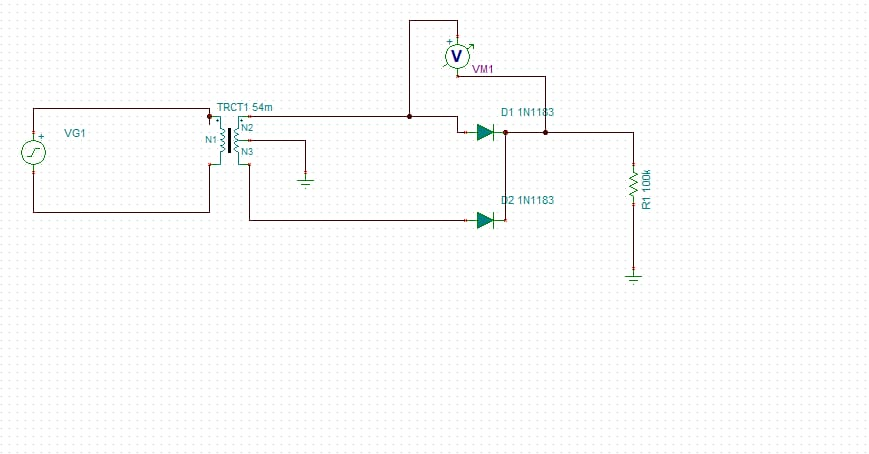
\includegraphics[width=12cm, height=6cm]{g1.png}
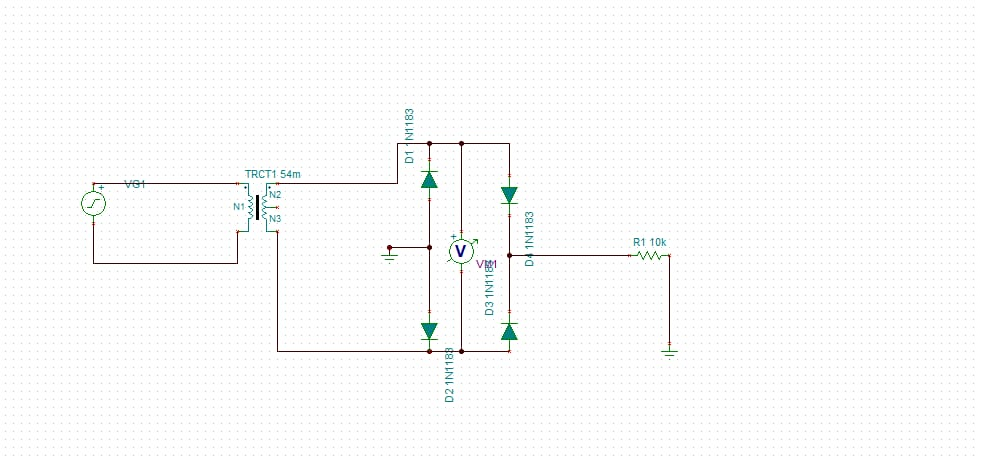
\includegraphics[width=12cm, height=6cm]{g2.png}
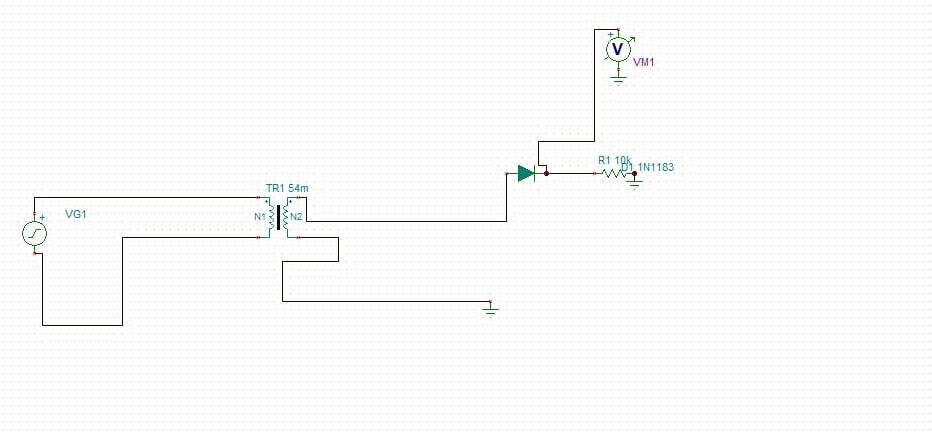
\includegraphics[width=12cm, height=6cm]{g3.png}
\end{center}
\end{figure}
\vspace{2cm}

\newpage
\begin{figure}
\paragraph{Gambar Percobaan Rangkaian di Osiloskop}
\paragraph{ }
\begin{center}
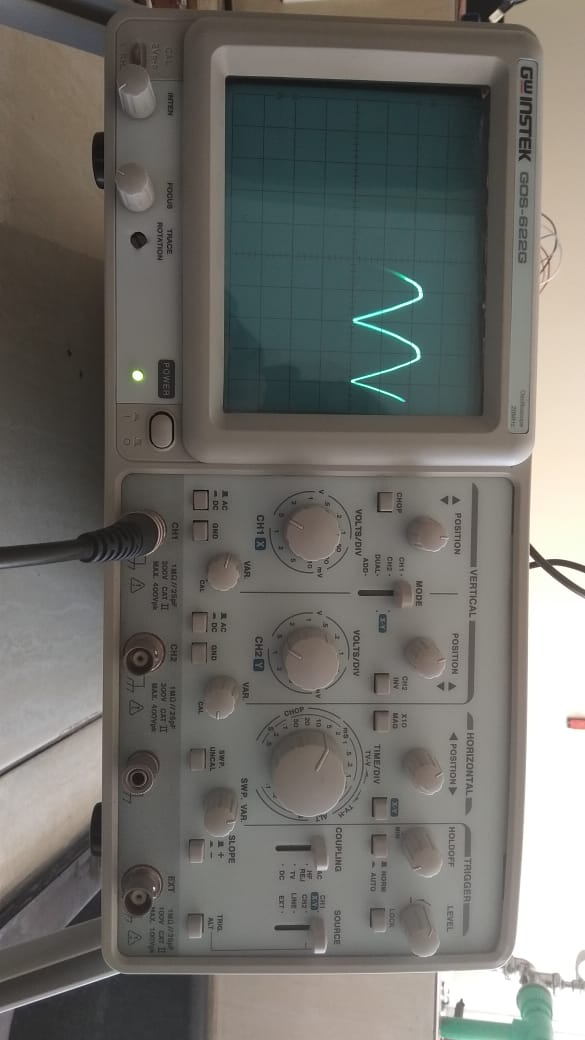
\includegraphics[width=6cm, height=12cm]{g4.png}
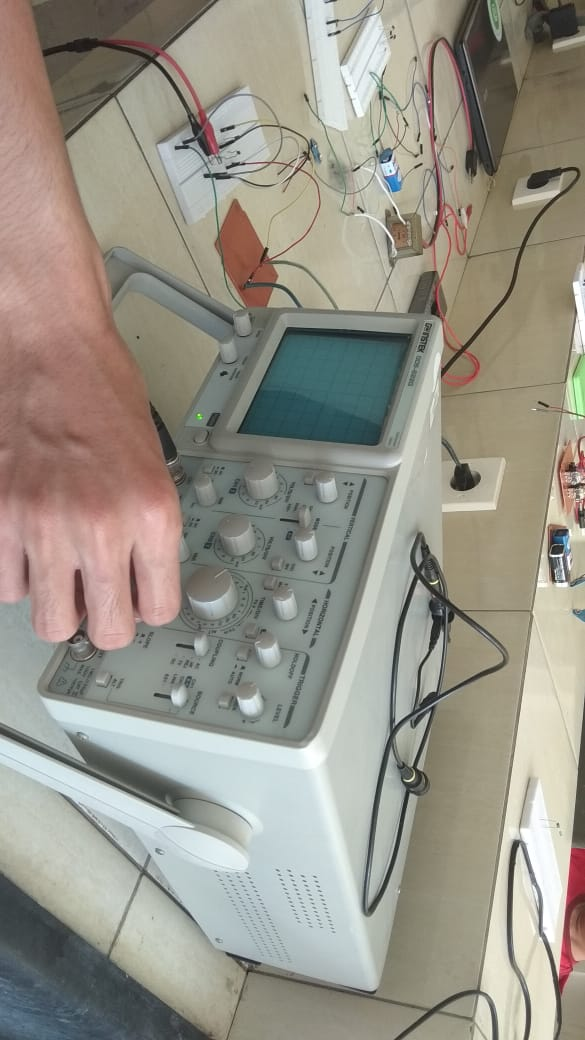
\includegraphics[width=6cm, height=12cm]{g5.png}
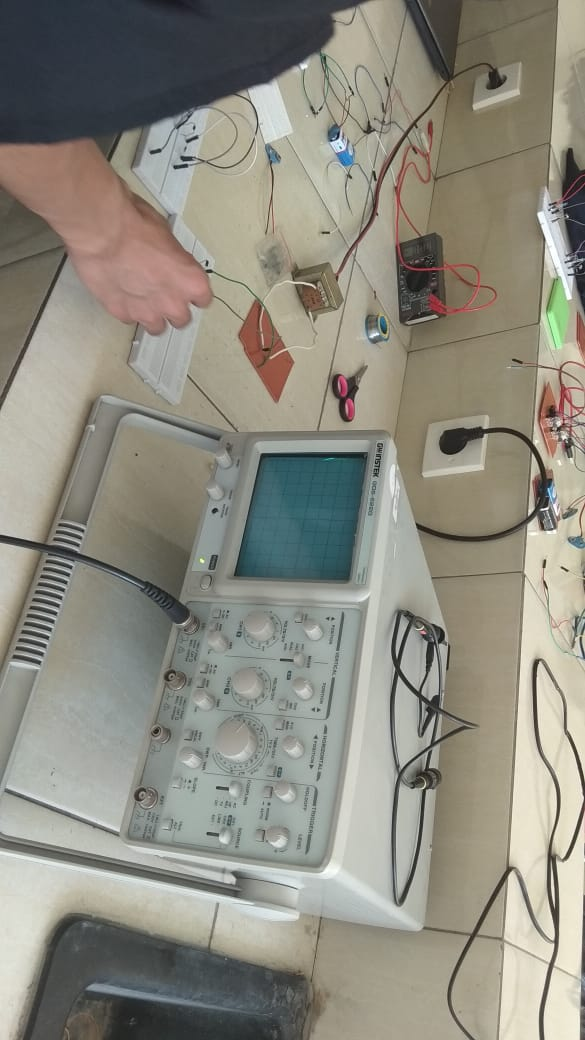
\includegraphics[width=6cm, height=12cm]{g6.png}
\end{center}
\end{figure}
\vspace{2cm}

\end{document} %Penulisan Laporan Berakhir
